\documentclass[11pt, a4paper]{report}

\usepackage{tikz}
\usetikzlibrary{decorations.pathmorphing}
\usetikzlibrary{decorations.markings}
\usetikzlibrary{positioning, shapes, snakes, arrows}

\begin{document}
\tikzset{
quark/.style={postaction={decorate}, decoration={markings,mark=at position .5 with {\arrow[#1]{latex}}}},
scalar/.style={dashed,postaction={decorate}, decoration={markings,mark=at position .5 with {\arrow[#1]{latex}}}},
gluon/.style={decorate, decoration={coil,amplitude=2pt, segment length=2pt,  pre length=.1cm, post length=.1cm}},
boson/.style={-latex,decorate, decoration={snake, segment length=4pt, amplitude=1.8pt, pre length=.1cm, post length=.25cm}},
%photon/.style={decorate, decoration={snake, segment length=4pt, amplitude=1.8pt,  pre length=.1cm, post length=.1cm}},
photon/.style={decorate, decoration={snake, segment length=4pt, amplitude=1.8pt}},
dphoton/.style={decorate, decoration={snake, segment length=4pt, amplitude=1.8pt,  pre length=.1cm, post length=.25cm},-latex}
}

%
%\begin{tikzpicture}[scale=1.5]
\begin{tikzpicture}[scale=2.5]
\def\wid{.7};
\def\iwid{.5};
%
\node (e1) at (1,1) [above] {1};
\node (e2) at (4,2) [above] {2};
\coordinate (e3) at (2,2.5);
\node (e4) at (1.3,4) [above] {4};
%


\draw [quark] (e1) -- (e3);
\draw [quark] (e3) -- (e4);
\draw [photon] (e3) -- (e2);

\end{tikzpicture}
%

%\begin{tikzpicture}[scale=1.5]
\begin{tikzpicture}[scale=2.5]
\def\wid{.7};
\def\iwid{.5};
%
\node (mu) at (-1,\wid) {$\mu^{+} (p)$};  
\node (e) at (-1,-\wid) {$e^{-} (q)$};
\coordinate (Wu) at (0,\iwid);
\coordinate (Wd) at (0,-\iwid);
\node (numu) at (1,\wid) {$\bar\nu_\mu (p')$}; 
\node (nue) at (1,-\wid) {$\nu_e (q')$};
%
\draw [fill=black] (Wu) circle (.04) node [above] {$\alpha$};
\draw [fill=black] (Wd) circle (.04) node [below] {$\beta$};
%
\draw [boson] (Wu) -- (Wd) node [midway, right] {$W^{+}$};

\draw [quark] (mu) -- (Wu);
\draw [scalar] (Wu) -- (numu);

\draw [gluon] (e) -- (Wd);
\draw [boson] (Wd) -- (nue);
%

\end{tikzpicture}

%
%\begin{tikzpicture}[scale=1.5]
\begin{tikzpicture}[scale=2.5]
\def\wid{.7};
\def\iwid{.5};
%
\node (mu) at (-1,\wid) {$\mu^{+} (p)$};  
\node (e) at (-1,-\wid) {$e^{-} (q)$};
\coordinate (Wu) at (0,\iwid);
\coordinate (Wd) at (0,-\iwid);
\node (numu) at (1,\wid) {$\bar\nu_\mu (p')$}; 
\node (nue) at (1,-\wid) {$\nu_e (q')$};
%
\draw [fill=black] (Wu) circle (.04) node [above] {$\alpha$};
\draw [fill=black] (Wd) circle (.04) node [below] {$\beta$};
%
\draw [boson] (Wu) -- (Wd) node [midway, right] {$W^{+}$};

\draw [quark] (mu) -- (Wu);
\draw [quark] (Wu) -- (numu);

\draw [photon] (e) -- (Wd);
\draw [dphoton] (Wd) -- (nue);
%

\end{tikzpicture}

%\begin{tikzpicture}[scale=1.5]
\begin{tikzpicture}[scale=2.5]

\draw [->,decorate,decoration={snake,amplitude=.4mm,segment length=2mm,post length=1mm}] (0,0) -- (3,0);

\end{tikzpicture}

    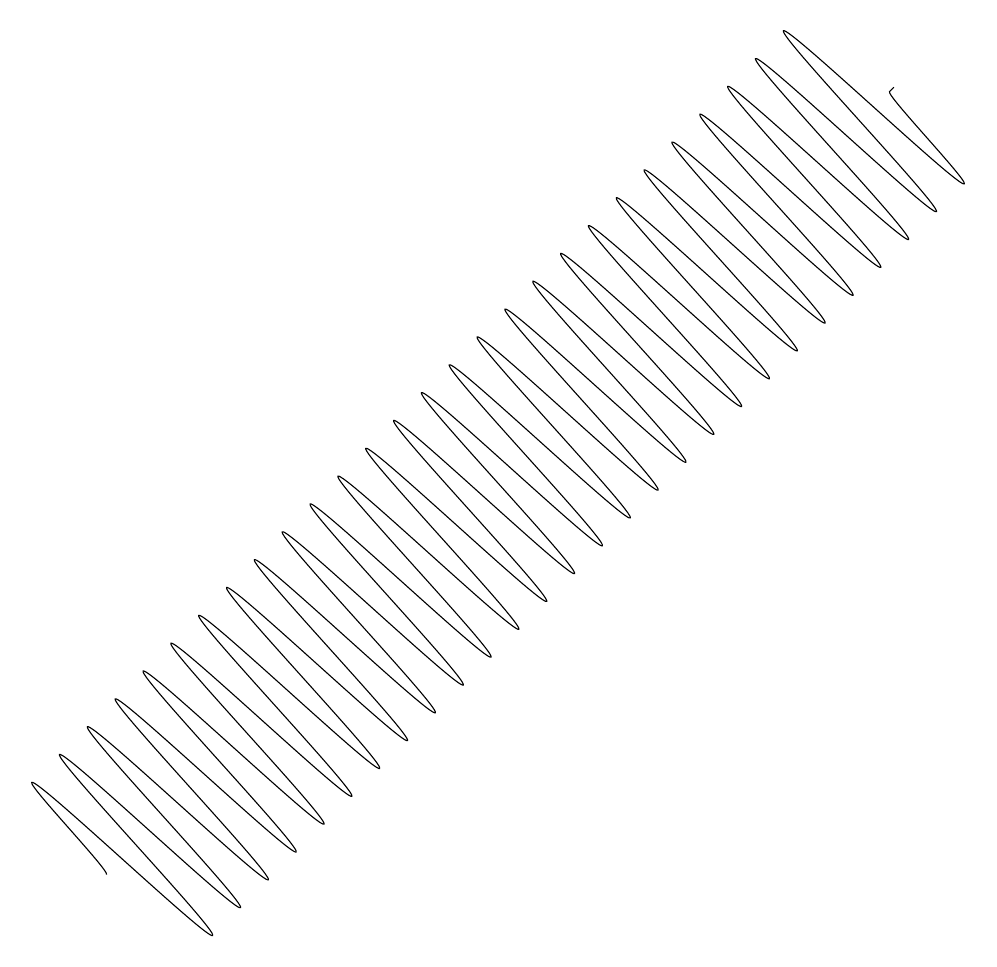
\begin{tikzpicture}
    %\draw[decorate, decoration=snake, segment length=5mm, amplitude=15mm] (0,0) -- (10,10);
    \draw[decorate, decoration={snake, segment length=5mm, amplitude=15mm}] (0,0) -- (10,10);
    \end{tikzpicture}


%\begin{tikzpicture}[scale=1.5]
\begin{tikzpicture}[scale=2.5]

\draw [->,decorate,decoration=snake] (0,0) -- (2,0);

\end{tikzpicture}

\end{document}
